\section{Algoritmo Dynamic Time Warping}
\label{sec:DTW}

Dynamic time warping, es una técnica que encuentra la alineación óptima entre dos series de tiempo, es un algoritmo para medir la similaridad entre dos secuencias, las cuales pueden variar en el tiempo o la velocidad.\\
Puede ser utilizado para encontrar regiones correspondientes entre las dos series o para determinar la similitud entre las dos series de tiempo.\\

Se utiliza a menudo en el reconocimiento de voz para determinar si dos formas de onda representan la misma frase hablada. En una forma de onda del habla, la duración de cada sonido hablado y el intervalo entre sonidos pueden variar, pero las formas de onda del habla deben ser similares.\\
También se ha encontrado útil en muchas otras disciplinas, incluyendo la minería de datos, reconocimiento de gestos, la robótica y la medicina \cite{DTW}.

La distancia euclidiana entre dos series de tiempo no es más que la suma de las distancias cuadradas de cada punto enésimo en una serie de tiempo hasta el punto enésimo en la otra.\\
El principal inconveniente de la utilización de la distancia euclidiana para datos de series de tiempo es que: si dos series de tiempo son idénticas, pero una se desplaza ligeramente a lo largo del eje de tiempo, entonces la distancia euclídea puede considerar que son muy diferentes la una de la otra.\\
DTW se introdujo para superar esta limitación, haciendo caso omiso de los cambios globales y locales en la dimensión de tiempo.\\

En general, el funcionamiento del algoritmo se basa en la búsqueda de un camino óptimo de coincidencia entre dos secuencias con ciertas restricciones. Las secuencias son transformadas no linealmente en el tiempo, de modo que son comprimidas o expandidas en el tiempo para que tengan el mismo largo, y así poder compararlas punto a punto. \\

\textbf{Algoritmo de alineamiento temporal dinámico:} \\

Supongamos que queremos comparar y evaluar la diferencia entre dos señales, supongamos que tenemos dos series de tiempo, un secuencia Q de longitud n, y una secuencia C de longitud m, donde: \\
Q = q1, q2, ..., qi, ..., qn 	(1)\\
C = c1, c2, ..., cj, ... cm 	(2)\\

Para alinear estas dos secuencias utilizando DTW, primero construimos una matriz de n por m,  $d(q_i,c_j) = d(q_i - c_j)^2$, que es la alineación entre los puntos  $q_i$ y $c_j$.\\
Para encontrar la mejor coincidencia entre estas dos secuencias, recuperamos un camino a través de la matriz que minimiza la distancia total acumulada entre ellos, como se ilustra en la Figura. En particular, la ruta óptima es el camino que minimiza el coste.\\

$DTW(Q,C)=min\left\{{\sqrt[]{\sum_{k=1}^K{w_k}}}\right\}$ \\

donde $w_k$ es el elemento de matriz $(i, j)_k$ que también pertenece al k-ésimo elemento de un camino de deformación $W$, un conjunto contiguo de elementos de la matriz que representan un mapeo entre $Q$ y $C$.\\

Este camino se puede encontrar utilizando programación dinámica para evaluar la siguiente repetición.\\
$ \gamma (i, j) = d (q_i, c_j) + min \left\{{\gamma (i-1, j-1), \gamma (i-1, j), \gamma (i, j-1)}\right\} $ \\

donde $d(i, j)$ es la distancia que se encuentra en la celda actual, y $\gamma (i, j)$ es la distancia acumulada de $d (i, j)$ y las distancias acumulativas mínimos de las tres células adyacentes.\\

\begin{figure}[h]%La h significa que la colocara cerca del texto
	\begin{center}
		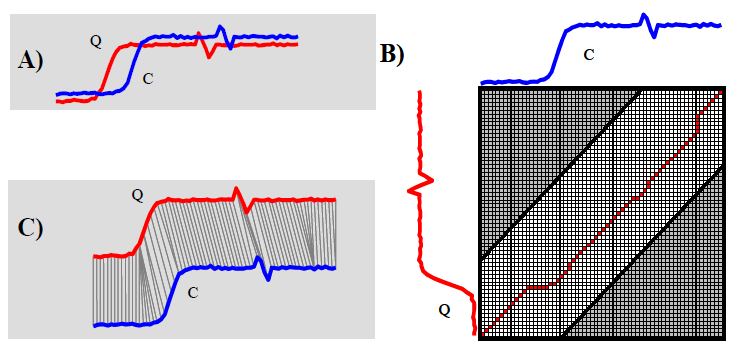
\includegraphics[scale=0.55]{./Figuras/DTWGraficas}
	\end{center}
	\caption{Comparación de dos señales de tiempo con DTW}
	\label{fig:comparacionsenalesdtw}
\end{figure}

La Figura (A) muestra dos secuencias similares Q y C, pero fuera de fase.\\
La Figura (B) para alinear las secuencias, se construye una matriz de deformación y la búsqueda de la ruta óptima, que se muestra con los cuadrados sólidos.\\
La Figura (C) muestra la alineación resultante.\\

Esta secuencia debe satisfacer tres condiciones:\\

1.-Condición de frontera: $p_l=(1,1)$ y $p_L=(N,M)$\\
   Para que los primeros  y los últimos elementos de X e Y estén alineados y así las secuencias completas estén alineadas.\\
   
2.-Condición de monotonía:  $n_1<= n_2<=...n_L $ y $ m_1 <= m_2 <= ... m_L$ \\
   Nos aseguramos de que elementos que se sucedan en el tiempo también se sucedan al ser alineados.\\
   
3.-Condición de salto: Nos indica que no se puede omitir ningún elemento de X e Y y que el camino de alineamiento es continuo.\\

Para reducir el número de rutas a considerar durante el cómputo, varias limitaciones conocidas (condiciones de frontera, la condición de continuidad, condición monótona y Ajuste Ventana Estado) se han aplicado al problema de restringir los movimientos que se pueden hacer desde cualquier punto la ruta de acceso y así restringir el número de caminos que necesitan ser considerados.\\

\clearpage

